\chapter{Software}
\par Este componente de software tendrá el propósito de asistir al fabricante de cerveza en las tareas de monitoreo, planificación y visualización de datos históricos de experimentos de maceración.

\par En los siguientes incisos, serán descriptas las consideraciones tomadas para la elección de una plataforma sobre la cual se desarrollará la aplicación de Software.

\section{Análisis de alternativas}
    \subsection{Tecnologías}
        \par A continuación se presenta una breve reseña de las plataformas actualmente más relevantes para dispositivos móviles.
        
        \subsubsection{Android}
            \par Android es un sistema operativo, el cual fue inicialmente desarrollado por Android Inc., empresa que Google respaldó económicamente y más tarde, en 2005, compró. Fue diseñado principalmente para dispositivos móviles con pantalla táctil desarrollados por Google o por terceros, como teléfonos inteligentes, tabletas y también, relojes inteligentes, televisores y automóviles. 
            
            \par Android es un sistema operativo basado en el núcleo Linux.
            
        \subsubsection{iOS}
            \par iOS es un sistema operativo móvil de la multinacional Apple Inc. Originalmente desarrollado para el iPhone (iPhone OS), después utilizado en dispositivos como el iPod touch y el iPad. No permite la instalación de iOS en hardware de terceros.
            
            \par iOS se deriva de macOS, que a su vez está basado en Darwin BSD, y por lo tanto es un sistema operativo Tipo Unix.
            
    \subsection{Comparación}
        \par El desarrollo será realizado para una plataforma móvil, de las cuales se tendrán en cuenta las siguientes consideraciones: cantidad de usuarios que la utilicen; tamaño de la comunidad a disposición para dar soporte; disponibilidad de mejores herramientas y utilidades para el desarrollo de aplicaciones.
        
        \par A continuación, se presenta una tabla comparativa en la cual se abordan aspectos de interés para la elección y un análisis concluyente.
        
        \begin{table}[h]
            \centering
            \begin{tabularx}{\textwidth}{|X|X|X|}
                 \hline
                 \multicolumn{3}{|c|}{Tabla comparativa de tecnologías de software}\\
                 \hline
                 Criterios de comparación & Android & iOS \\
                 \hline
                 \hline
                 
                 Porcentaje Mercado (Arg) & 75\% & 19\%  \\
                 \hline
                 
                 Porcentaje Mercado Internacional & 85\% & 14,7\% \\
                 \hline
                 
                 Comunidad de desarrolladores & Muy grande & Amplia pero acorde al número de usuarios\\
                 \hline
                 
                  Entornos desarrollo Propia & Android Studio & Xcode\\
                 \hline
                 
                 Lenguaje de desarrollo & Java, C, C++ y Kotlin & Swift, C, C++ y objective-C\\
                 \hline
                 
                 Familia del SO & Linux & Unix - BSD\\
                 \hline
                 
                 Complejidad de desarrollo & Muy diversa variedad de dispositivos y de versiones del SO & Variedad reducida de dispositivos, versiones de SO comunes a la mayoría\\
                 \hline
                 
                 Entorno & Open Source & Entorno cerrado \\
                 \hline
                 
                 Requerimientos para publicación de aplicación & Ninguna & Debe cumplir requisitos de Apple\\
                 \hline
                 
            \end{tabularx}
            \caption{Comparación de plataformas móviles}
            \label{tab:ComparacionPlataformasMoviles}
        \end{table}

    
    \subsection{Elección}
    \par
    La elección fue realizada a partir de los criterios antes mencionados aplicados sobre la tabla comparativa.
    \par
    Se decidió desarrollar la aplicación para la plataforma \textbf{Android}, considerado, el porcentaje de uso en Argentina, el tamaño de la comunidad de desarrolladores, la gran disponibilidad de herramientas y la sencillez relativa en cuanto a requerimientos para la publicación de aplicaciones.
    
    \par Para el desarrollo se empleó el lenguaje Java (JDK 1.7 o Java 7) sobre el entorno de desarrollo integrado (IDE) oficial de Google, AndroidStudio. La versión de sistema operativo mínima para la que se desarrolló es \textit{Nougat 7.0}, lanzada en agosto de 2016, la cual utiliza la plataforma de desarrollo (Android SDK plataform \footnote{\url{https://developer.android.com/studio/releases/platforms}}) API nivel 24.




\section{Diseño}
    \subsection{Diseño de la interfaz de usuario}
        \par Las figuras \ref{fig:MockUpMainActivity}, \ref{fig:MockUpPlanningActivity}, \ref{fig:MockUpExperimentActivity}, \ref{fig:MockUpInfoMash}, \ref{fig:MockUpCurrentExperienceFragment}, \ref{fig:MockUpStageFragment}, \ref{fig:MockUpGeneralFragment} y \ref{fig:MockUpExperimentFragment} ubicadas en el Anexo, diagraman y describen el diseño y las funcionalidades de la interfaz de usuario (UI) bosquejadas para la aplicación móvil.
        
    \subsection{Diagrama de Clases}
    \par
    En el anexo, Figura 9, puede encontrar el diseño diagrama de clases  un diagrama de clases  de la aplicación.
    
    \subsection{Base de Datos}
        \par En el siguiente diagrama (Figura \ref{fig:DiagramaBdApp}) se esquematiza la base de datos a alojar en la aplicación. En el diagrama se pueden distinguir las tablas a utilizar para la abstracción de la aplicación y el conjunto de relaciones establecidas entre ellas.
        
        \begin{figure}[h]
            \centering
            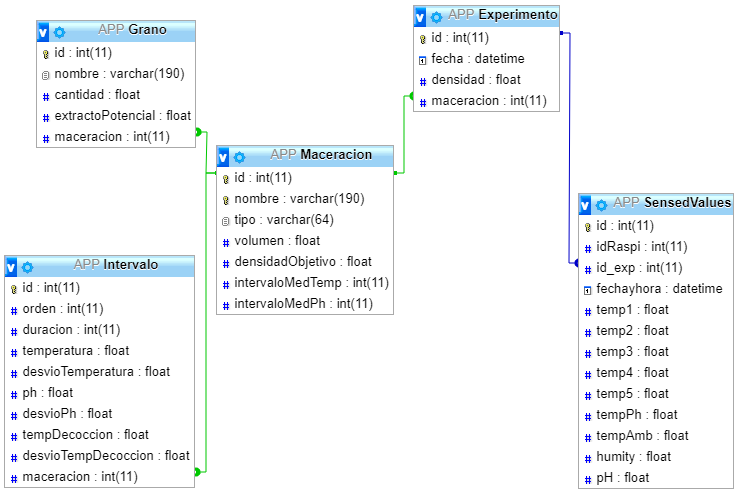
\includegraphics[scale=0.8]{DiagramaBaseDeDatosAPP.jpg}
            \caption{Diagrama de Base de Datos de la aplicación}
            \label{fig:DiagramaBdApp}
        \end{figure}

\section{Implementación}
    \par Esta sección contiene la presentación de los resultados obtenidos del desarrollo de este componente. 
    El desarrollo de esta aplicación [fue realizado utilizando principalmente el lenguaje java junto al IDE  Android Studio.
    de desarrollo AndroidStudio (LO DE ANDROID STUDIO Y VERSION DE JAVA LO PUSE ARRIBA)] se basa en el patrón de arquitectura de desarrollo MVP \footnote{MVP, Modelo Vista Presentador. Patrón que separa la lógica de datos y de negocios(modelo y presentador respectivamente) de la interfaz gráfica (Vista)}. Los elementos correspondientes a la lógica    
    

    
    se divide en ciertos elementos denominados \textit{Activities}, los cuales incluyen componentes de interfaz gráfica denominados Vistas(\textit{Views}) y los eventos correspondientes a la interacción con los mismos (patrón \textit{observer}). 
    
    \par Debido a la imposibilidad de la desagregación de ciertas funciones, los \textit{activities} incluyen métodos o llamadas que interaccionan con librerías o clases complementarias. Dentro de estas últimos se encuentran el modelo de clases, la interacción con la base de datos y llamadas a las API's, entre otras.
    
    \par Para cada uno de los \textit{activities} de la misma se adjunta la correspondiente descripción general, las funciones que cumple y interacción con clases o librerías complementarias. 
    
    
        \subsection{Pantalla principal}
        
            \subsubsection{Descripción}
                \par Es la pantalla con la que inicia la aplicación. En la misma se puede visualizar la lista de maceraciones planificadas.
                
                \par Para la implementación se utiliza un Activity denominado \textit{MainActivity}. La interfaz definida se compone por un ActionBar que cuenta con un botón para acceder a la pantalla de planificación, una lista de elementos (maceraciones) que ocupa el área restante de la pantalla (RecyclerView?, Adapter?) y un botón flotante para acceder un dialogo tipo pop up donde puede observarse los valores actuales recolectados por los sensores de la estación de recolección de datos Figura X. 
                
            \subsubsection{Funciones}
                \paragraph{Lista de maceraciones planificadas:}
                Cada una de las maceraciones listadas es un botón clickeable que permite el acceso a la pantalla de gestión de la maceración seleccionada.
                \paragraph{Agregar nueva maceración:}
                Al seleccionar el botón, se accede a la pantalla que permite crear una nueva maceración.
                \paragraph{Medición actual:}
                Dialogo pop up que muestra los valores obtenidos por cada sensor, Figura X.
            
            \subsubsection{Detalle de implementación}
                En el diagrama X ubicado en el Anexo, pueden observarse las clases y funciones utilizadas para el despliegue de esta pantalla.
                
                
        \subsection{Pantalla de planificación}
        \subsubsection{Descripción}
                \par Es la pantalla donde se planifica una nueva maceración. En la misma se pueden visualizar opciones para rellenar los campos necesarios para definir una maceración.
                
                \par Para la implementación se utiliza un Activity denominado \textit{PlanningActivity}. La interfaz definida se compone por un actionbar que cuenta con un botón para finalizar la planificación, una lista de campos (tipo de maceración, volumen, densidad deseada, lista de granos, lista de intervalos) que ocupa el área restante de la pantalla. 
                
            \subsubsection{Funciones}
                \paragraph{Seleccionar tipo de maceración:}
                Menú desplegable que permite seleccionar el tipo de maceración de una lista predefinida, siendo estas opciones \textit{simple}, \textit{escalonada} o \textit{por decocción}.
                
                \paragraph{Establecer volumen y densidad deseada:}
                Estos parámetros se pueden establecer rellenando los campos correspondientes. El volumen ingresado debe estar expresado en litros y la densidad en kilogramos sobre litro.
                
                \paragraph{Agregar/Quitar granos:}
                Al presionar el botón ``AGREGAR GRANO'', se despliega un dialogo con tres campos, Figura X,  donde se deberá agregar el nombre del grano, porcentaje correspondiente a la receta y el extracto potencial provisto por el fabricante del mismo. Una vez agregado, los datos del mismo se mostrarán en una lista en conjunto con los granos agregados anteriormente.
                \par Para eliminar un elemento de esta lista, se debe mantener presionado el mismo y seleccionar la opción ``Eliminar grano'' del menú contextual (Figura X).
                
                \paragraph{Definir intervalos con sus parámetros:}
                Para el agregado de intervalos debe seleccionarse el botón con el signo ``+'', esto desplegará un dialogo tipo pop-up, Figura X, donde podrán encontrarse los campos necesarios para definir un intervalo. Pueden ser agregados uno o mas intervalos según corresponda al tipo y receta de maceración a ser realizada.
                
                \paragraph{Finalizar planificación:}
                Al finalizar el ingreso de datos, ser presionará el botón para finalizar, antes mencionado, esto desplegará un dialogo tipo pop-up donde deberán ser ingresados los campos nombre de la maceración, intervalo de medición de temperatura e intervalo de medición de pH. Luego del ingreso de los datos, presionando el botón ``Aceptar'' dará por concluido el ingreso de datos y se retornará al \textit{Main Activity}.
                
                \paragraph{Regla de negocios}
                Dado que es necesario mantener igualdad de condiciones para los experimentos de maceración llevados a cabo con los parámetros aquí ingresados, los mismos no podrán ser modificados luego. Debiendo en el caso de requerir modificarlos, eliminar la maceración e ingresar nuevamente los datos.
            
            \subsubsection{Detalle de implementación}
                En el diagrama X ubicado en el Anexo, pueden observarse las clases y funciones utilizadas para el despliegue de esta pantalla.
        
        \subsection{Pantalla de gestión de maceración}
            \subsubsection{Descripción}
                \par Es la pantalla de administración para la maceración seleccionada.
                \par Para la implementación se utiliza un Activity denominado \textit{ExperimentActivity}. En la misma puede ser visualizado en primer lugar un ActionBar donde se indica el nombre de la maceración y que incluye además una serie de botones: acceso a la pantalla de detalle de la maceración, ingreso a la pantalla de información histórica y estadística de los experimentos realizados, y por último, la opción de eliminar la maceración. En el área restante de la pantalla puede encontrarse una lista con los experimentos realizados, y un botón flotante en la parte inferior que permite iniciar un nuevo experimento y acceder de esta manera a la pantalla correspondiente.
                
                
            \subsubsection{Funciones}
                \paragraph{Lista de experimentos realizados:}
                Cada una de los experimentos listados es un botón sensible a ser presionado que permite el acceso a la pantalla de resultados del experimento pulsado (Figura X).
                
                \paragraph{Eliminar experimento:}
                 Como se mencionó en el punto anterior, cada una de los experimentos listados es un botón sensible a ser presionado. Si la duración de esta selección supera los dos segundos, se procede a borrar el experimento seleccionado de la lista y de la base de datos.
                 
                \paragraph{Detalle del plan de maceración:}
                 Pantalla en la cual pueden ser visualizados los valores ingresados en la planificación de la maceración; el volumen y temperatura de agua a ser incorporada en cada etapa; y la cantidad de cada tipo de grano a ser utilizado.
                
                \paragraph{Información histórica y estadística:}
                Acceso a la pantalla de información histórica y estadística correspondiente a la maceración. (Figura X)
                
                \paragraph{Eliminar maceración:}
                Al seleccionarse la opción presente en el ActionBar, se procede a eliminar la maceración actual en conjunto con todos los datos ligados a la misma (experimentos realizados y datos inherentes a la planificación de la misma)
                
                \paragraph{Iniciar nuevo experimento}
                Ingreso a la pantalla de monitoreo del experimento a ser iniciado (Figura X).
            
            \subsubsection{Detalle de implementación}
                En el diagrama X ubicado en el Anexo, pueden observarse las clases y funciones utilizadas para el despliegue de esta pantalla.
            
        \subsection{Pantalla de detalle de maceración}
            \subsubsection{Descripción}
            Es la pantalla donde se presentan los datos ingresados para esta maceración en la planificación, junto a otros datos calculados.
            En la misma puede ser visualizarse en la parte superior el \textit{ActionBar} donde se indica el nombre de la Maceración. Luego, en el espacio restante se presentan los siguientes valores: tipo de maceración; volumen de mosto; densidad específica deseada; información de los granos a utilizar (nombre, cantidad teórica y, en caso de haber realizado mas de tres experimentos, la cantidad ajustada); e información de los intervalos (duración, temperatura y pH deseados con sus respectivas tolerancias de desvío, volumen y temperatura del agua a ser incorporada, y en caso de maceración por decocción, la temperatura del segundo macerador).
            
            \subsubsection{Detalle de implementación}
            
        \subsection{Pantalla de información estadística e histórica}
            \subsubsection{Descripción}
            En esta pantalla puede ser visualizado un resumen de los experimentos llevados a cabo para la correspondiente maceración.
            En esta pantalla puede visualizarse un \textit{ActionBar} en la parte superior con el nombre de la maceración. Debajo, dos botones tipo pestañas (\textit{TabLayout}) que permiten acceder a los dos paneles (\textit{Fragments}), Resumen General y Detalle de temperatura de cada experimento. 
            Se divide en dos paneles (\textit{Fragments}): Resumen general y Detalle de temperatura por experimento.
            
            \paragraph{Resumen general:} En este panel en primer lugar se ubica un botón que permite alternar entre los dos tipos de gráficas comparativas de la evolución promedio de cada variable (gráfica de líneas y gráfico estadístico descriptivo Boxplot\footnote{También conocido como gráfico de caja y bigote (representa valores extremos y el 1$^{\circ}$, 2$^{\circ}$ y 3$^{\circ}$ cuartil)}). Luego de este, se presentan las siguientes gráficas: Temperatura; pH; y Activación de enzimas. Finalmente, se presenta una serie de valores calculados a partir de los mismos valores que conforman las gráficas, estos son: Número de experimentos válidos; Rendimiento del equipo\footnote{Este valor comienza a ajustarse a partir del tercer experimento válido de una maceración}; Cálculo Teórico de insumos con rendimiento no ajustado \footnote{El ajuste se realiza tomando como rendimiento del equipo el valor de rendimiento calculado, en lugar del estándar 70\%}; Cálculo Teórico de insumos con rendimiento ajustado; por último el calculo práctico de cantidad de insumos. 
            
            \paragraph{Detalle de temperatura por experimento:} En este puede encontrarse en el borde superior un menú desplegable (\textit{Spinner}), el cual permite seleccionar el tipo de gráficas a ser comparadas luego, pudiendo ser de cada sensor o del promedio de sensores para cada muestra. De esta manera permite compara el/los mismo/s sensores entre diferentes experimentos. Debajo, se presentan las gráficas por experimento antes mencionadas.
            
            \subsubsection{Funciones}
            \paragraph{Visualización de gráficas de variables:}
              En el resumen general, se presentan gráficas de los valores promedios de las variables antes mencionadas respecto al tiempo. Se consideran para estas solo los experimentos válidos\footnote{Se consideran válidos aquellos experimentos, que cumplan con la cantidad de mediciones e incluyan el valor de densidad obtenida.} de esta maceración.
            
            \subsubsection{Detalle de implementación}
            
        \subsection{Pantalla de resultados de experimento}
            \subsubsection{Descripción}
            En esta pantalla puede ser viualizado un resumen de los resultados obtenidos en este experimento.
            En el borde superior se ubica un \textit{ActionBar} con el la fecha y horario del experimento, debajo se presentan los valores temperatura ambiental, densidad específica del mosto y rendimiento obtenido. En forma posterior, se ubican representaciones gráficas de la evolución temporal de las variables temperatura, pH y activación de enzimas para este experimento, seguidas de la evolución temporal de la temperatura de cada sensor.
            
            \subsubsection{Detalle de implementación}
            
        \subsection{Pantalla de monitoreo de experimento}
            \subsubsection{Descripción}
            Esta pantalla es la encargada de asistir al usuario con el experimento en curso.
            En esta pantalla puede visualizarse un \textit{ActionBar} en la parte superior con el nombre de la maceración, seguido de dos botones, el primero para cancelar el experimento en curso y el segundo para confirmar la conclusión del experimento. Debajo, dos botones tipo pestañas (\textit{TabLayout}) que permiten acceder a los dos paneles (\textit{Fragments}), Mediciones y Etapas.
            
            \paragraph{Mediciones:}
            En este panel se visualizan los valores obtenidos a través de la estación de recolección de datos para el experimento en curso. Además, enseña dentro de tarjetas (\textit{CardViews}) el porcentaje de avance en el que se encuentre la maceración, los valores planificados para dicho momento y el correspondiente desvío con los valores recolectados.
            \paragraph{Etapas:}
            En este panel se visualiza un resumen de las etapas que componen la maceración, adicionando temporizadores correspondientes al tiempo restante para el inicio de cada una de las mismas.
            
            \subsubsection{Funciones}
            \paragraph{Configuración de medición de temperatura:} Manteniendo presionada la tarjeta perteneciente a la temperatura, se abre un dialogo de selección, el cual permite elegir los métodos de representación de los valores de temperatura para monitoreo. Estos pueden ser: promedio, mediana, promedio de valores extremos, y finalmente permite seleccionar los sensores incoroporados o exceptuados del cálculo.
            \paragraph{Alerta:} 
            En caso de obtenerse un valor fuera de la tolerancia planificada, se muestra una notificación en el dispositivo correspondiente a la variable fuera de rango. 
            \paragraph{Finalizar experimento:}
            Al seleccionar esta opción, en caso que se hayan realizado todas las mediciones del experimento, se muestra un dialogo para que el usuario ingrese el valor de densidad especifica del mosto obtenida. En caso de no haber completado las mediciones, se enseña un mensaje indicando dicha situación.
            \paragraph{Cancelar experimento:} 
            Esta función permite abortar el experimento en curso. Una vez cancelado, se procede a la eliminación de todos los datos relacionados al experimento cancelado.
            
            \subsubsection{Detalle de implementación}
            